\documentclass[12pt,a4paper]{article}
\usepackage[utf8]{inputenc}
\usepackage[T1]{fontenc}
\usepackage{ngerman}
% german support inline
\usepackage{geometry}
\geometry{a4paper, margin=2.5cm}
\usepackage{setspace}
\usepackage{amsmath, amssymb, amsthm}
\usepackage{mathtools}
\usepackage{pgfplots}
\pgfplotsset{compat=1.18}
\usepackage{tikz}
\usetikzlibrary{shapes.geometric, arrows.meta, positioning, fit, backgrounds, calc}
\usepackage{booktabs}
\usepackage{array}
\usepackage{multirow}
%\usepackage{microtype}
\usepackage{graphicx}
\usepackage{caption}
\usepackage{rotating}
\usepackage{subcaption}
\usepackage{microtype}
\usepackage{rotating}
\usepackage{float}
\usepackage{hyperref}
\hypersetup{
	colorlinks=true,
	linkcolor=blue!60!black,
	citecolor=green!50!black,
	urlcolor=blue,
	pdftitle={Innovativer Motorraum-Entwurf fuer Verbrennungs- und Elektrofahrzeuge},
	pdfauthor={Stephan Epp},
}
\usepackage{algorithm2e}
\usepackage{listings}
\usepackage{xcolor}
\usepackage{enumitem}
\usepackage{fancyhdr}
\usepackage{titlesec}
\usepackage{abstract}
\usepackage{tocloft}
\usepackage{enumitem}
\setlist[itemize,1]{label=--}

% --- Theoreme ---
\newtheorem{theorem}{Theorem}[section]
\newtheorem{lemma}[theorem]{Lemma}
\newtheorem{corollary}[theorem]{Korollar}
\newtheorem{proposition}[theorem]{Proposition}
\newtheorem{definition}{Definition}[section]
\newtheorem{remark}{Bemerkung}[section]

% --- Farben ---
\definecolor{mainblue}{RGB}{0,70,140}
\definecolor{accentred}{RGB}{180,30,30}
\definecolor{codegreen}{rgb}{0,0.6,0}
\definecolor{codegray}{rgb}{0.5,0.5,0.5}
\definecolor{backcolour}{rgb}{0.97,0.97,0.97}

\lstdefinestyle{pythonstyle}{
	backgroundcolor=\color{backcolour},
	commentstyle=\color{codegreen},
	keywordstyle=\color{mainblue},
	numberstyle=\tiny\color{codegray},
	stringstyle=\color{accentred},
	basicstyle=\ttfamily\footnotesize,
	breaklines=true,
	numbers=left,
	frame=single,
	language=Python
}

% ============================================================
\begin{document}
% ============================================================

% --- Titelseite ---
\begin{titlepage}
	\centering
	\vspace*{1.5cm}
	\vspace{0.5cm}
	{\Huge\bfseries
		Innovativer Motorraum-Entwurf für Kraftfahrzeuge
		\par}
	{\large\itshape
		Formaler Entwurf zugänglichkeitsoptimierter Motorräume für\\
		Verbrennungsmotoren (Diesel/Benzin) und Elektrofahrzeuge\\
		unter Einbeziehung eines KI-gesteuerten Batteriemanagementsystems
		\par}
	\vspace{1.5cm}
	{\large
		\begin{tabular}{rl}
			\textbf{Autor:}      & Stephan Epp \\[4pt]
			\textbf{Datum:}      & 9. März 2026 \\[4pt]
		\end{tabular}
	}
\end{titlepage}

% --- Abstract ---
\begin{abstract}
	\noindent
	Der Motorraum eines Kraftfahrzeugs stellt eine der komplexesten Integrationszonen
	im Fahrzeugbau dar: Mehrere Dutzend Subsysteme müssen auf engem Raum sicher
	koexistieren, thermisch entkoppelt werden und für Wartung, Diagnose und
	Notfallzugang erreichbar bleiben. Klassische Motorräume werden überwiegend
	bauraumgetrieben entworfen -- Zugänglichkeit wird nachgelagert berücksichtigt.

	Diese Arbeit präsentiert einen formalen, zugänglichkeitsorientierten Entwurfsrahmen
	für zwei fundamentale Motorraum-Architekturen: \textbf{(A)} Verbrennungsmotor-Fahrzeuge
	(Diesel und Benzin) und \textbf{(B)} Elektrofahrzeuge (EV) mit Lithium-Ionen-Batterien.
	Für Architektur~(B) werden die Ergebnisse eines formal bewiesenen KI-gesteuerten
	Power-Management-Moduls (AI-PMM) \cite{Epp2026liion} direkt in geometrische
	und thermische Entwurfsprinzipien übersetzt: maximale Erreichbarkeit der
	Batterie, ihrer Sensorik und Kühlsysteme ist zwingende Voraussetzung für den
	adaptiven Betrieb des AI-PMM.

	Es wird ein quantitatives Erreichbarkeitsmaß $\mathcal{A}$ definiert und
	gezeigt, dass ein topologisch optimierter Motorraum das Erreichbarkeitsmaß
	gegenüber einem konventionellen Layout um den Faktor $\Phi_\mathcal{A} \geq 2{,}3$
	steigert. Für EV-Architekturen wird ein Sicherheits- und Wartungskorridor-Konzept
	vorgestellt, das thermische Entkopplung, Hochvoltschutz und vollständige
	Zugänglichkeit aller AI-PMM-relevanten Komponenten vereint. Formale Stabilitäts-
	und Zugänglichkeitsbeweise sowie Simulationsergebnisse belegen die Überlegenheit
	des vorgestellten Entwurfs.
\end{abstract}

\vspace{1cm}
\noindent\textbf{Schlüsselwörter:} Motorraum-Entwurf, Zugänglichkeitsoptimierung,
Verbrennungsmotor, Elektrofahrzeug, Lithium-Ionen-Batterie, KI-Power-Management,
thermische Entkopplung, Hochvoltarchitektur, Wartungskorridor, Topologieoptimierung.

\newpage
\tableofcontents
\newpage

% ============================================================
\section{Einleitung}
% ============================================================

\subsection{Motivation und Problemstellung}

Der Motorraum eines modernen Kraftfahrzeugs ist eine der dichtest besiedelten
Systemzonen in der Fahrzeugtechnik. Auf einem Volumen von typischerweise
$0{,}3\text{--}0{,}8\,\mathrm{m^3}$ müssen Antriebsaggregat, Kühlung,
Hochspannungskomponenten (bei EV), Steuergerätenetzwerk, Fluidsysteme und
Sensorik koexistieren. Gleichzeitig stellen Wartbarkeit, Notfallzugang und
die zunehmende Systemdichte für Elektrofahrzeuge fundamental neue Anforderungen
an die Raumordnung des Motorraums.

Klassische Entwurfsmethoden orientieren sich primär an Bauraumrestriktionen
und Crashpfadgeometrien -- Zugänglichkeit wird als nachgelagertes Kriterium
behandelt \cite{Heißing2013}. Diese Arbeit kehrt die Priorität um:
\textit{Zugänglichkeit ist ein primäres Entwurfsziel}, das die gesamte
topologische Struktur des Motorraums bestimmt.

Für Elektrofahrzeuge gewinnt diese Perspektive eine neue Qualität: Das in
\cite{Epp2026liion} formal bewiesene KI-gesteuerte Power-Management-Modul
(AI-PMM) für Lithium-Ionen-Batterien erfordert physischen Zugang zu Zellsensorik,
Kühlkreisläufen und Hochvoltschnittstellen für Kalibrierung, Diagnose und
Im-Betrieb-Parametrierung. Ein Motorraum, der diese Zugänglichkeit nicht
geometrisch verankert, verhindert den optimalen Betrieb des AI-PMM und
damit die nachgewiesene Lebensdauerverlängerung um den Faktor $\Phi \geq 1{,}47$
\cite{Epp2026liion}.

\subsection{Zielsetzung und Beitrag}

Diese Arbeit leistet folgende wissenschaftliche Beiträge:

\begin{itemize}[leftmargin=*]
	\item Formale Definition eines Erreichbarkeitsmaßes $\mathcal{A}$ für
	Kraftfahrzeug-Motorräume unter Berücksichtigung von Sicherheits- und
	Geometrieconstraints.
	\item Entwurf eines zugänglichkeitsoptimierten Motorraum-Layouts für
	Verbrennungsmotor-Fahrzeuge (Diesel/Benzin) als Referenzarchitektur~(A).
	\item Entwurf einer AI-PMM-kompatiblen EV-Motorraum-Architektur (B) mit
	formaler Ableitung der Zugänglichkeitsanforderungen aus den Ergebnissen
	von \cite{Epp2026liion}.
	\item Quantitativer Nachweis der Zugänglichkeitsüberlegenheit beider
	Architekturen gegenüber konventionellen Layouts.
	\item Thermische Analyse und formale Stabilitätsaussagen für die
	Kühlsystemarchitektur beider Varianten.
\end{itemize}

\subsection{Aufbau der Arbeit}

Abschnitt~\ref{sec:grundlagen} legt die geometrischen, thermischen und
sicherheitstechnischen Grundlagen des Motorraum-Entwurfs dar. Abschnitt~\ref{sec:erreichbarkeit}
formalisiert das Erreichbarkeitsmaß. Abschnitt~\ref{sec:architektur_a} beschreibt
den optimierten Motorraum für Verbrennungsmotor-Fahrzeuge. Abschnitt~\ref{sec:architektur_b}
entwickelt die EV-Architektur unter Einbeziehung der AI-PMM-Anforderungen.
Abschnitt~\ref{sec:beweis} erbringt den formalen Erreichbarkeitsbeweis.
Abschnitt~\ref{sec:thermik} analysiert das thermische Verhalten beider Architekturen.
Abschnitt~\ref{sec:simulation} präsentiert Simulationsergebnisse, und
Abschnitt~\ref{sec:fazit} schließt mit Fazit und Ausblick.

% ============================================================
\section{Grundlagen des Motorraum-Entwurfs}
\label{sec:grundlagen}
% ============================================================

\subsection{Geometrische Grundprinzipien}

\subsubsection{Motorraum-Topologie}

Ein Motorraum $\mathcal{M}$ wird als kompakter metrischer Raum mit Randbedingungen
modelliert:

\begin{definition}[Motorraum-Topologie]
	Der Motorraum $\mathcal{M} \subset \mathbb{R}^3$ ist ein beschränktes,
	zusammenhängendes Volumen mit:
	\begin{equation}
		\mathcal{M} = \mathcal{V}_\mathrm{gesamt} \setminus
		\left(\bigcup_{i=1}^{N} \mathcal{V}_i^\mathrm{Komp}\right)
		\label{eq:motorraum_top}
	\end{equation}
	wobei $\mathcal{V}_i^\mathrm{Komp}$ die Belegungsvolumina der $N$ eingebauten
	Komponenten bezeichnet und $\mathcal{M}$ das verbleibende Zugänglichkeitsvolumen.
\end{definition}

Die Gesamtvolumenbilanz lautet:

\begin{equation}
	V_\mathrm{gesamt} = \sum_{i=1}^{N} V_i^\mathrm{Komp} + V_\mathrm{Zugängl.}
	+ V_\mathrm{Sicherheit} + V_\mathrm{Thermik}
	\label{eq:volumenbilanz}
\end{equation}

Für konventionelle Motorräume gilt typischerweise:
$V_\mathrm{Zugängl.}/V_\mathrm{gesamt} \approx 0{,}12\text{--}0{,}18$,
was auf die geringe Priorisierung der Zugänglichkeit im klassischen Entwurf
hinweist.

\subsubsection{Komponentenhierarchie}

Die $N$ Komponenten werden nach Austauschhäufigkeit und Zugänglichkeitsdringlichkeit
in drei Prioritätsklassen eingeteilt:

\begin{definition}[Zugänglichkeitsklassen]
	\begin{align}
		\mathcal{C}_1 &= \{\text{Tagesinspektion, Betriebsflüssigkeiten, Diagnoseschnittstellen}\}
		\label{eq:klasse1} \\
		\mathcal{C}_2 &= \{\text{Wartung \,<\,50\,000\,km: Filter, Riemen, Kühler}\}
		\label{eq:klasse2} \\
		\mathcal{C}_3 &= \{\text{Großreparatur, Grundaggregat-Zugang}\}
		\label{eq:klasse3}
	\end{align}
\end{definition}

Das Entwurfsprinzip verlangt: $\mathcal{C}_1$-Komponenten müssen ohne Werkzeug
erreichbar sein ($d_\mathrm{Zugang} \leq 300\,\mathrm{mm}$ Handtiefe);
$\mathcal{C}_2$-Komponenten mit Standardwerkzeug ($d \leq 600\,\mathrm{mm}$);
$\mathcal{C}_3$-Komponenten bei vollständig geöffnetem Motorraum.

\subsection{Thermische Grundlagen}

\subsubsection{Wärmezonierung}

Der Motorraum wird in thermische Zonen $\mathcal{Z}_k$ unterteilt:

\begin{equation}
	\mathcal{M} = \bigsqcup_{k=1}^{K} \mathcal{Z}_k, \quad
	\mathcal{Z}_k \cap \mathcal{Z}_l = \emptyset \text{ für } k \neq l
	\label{eq:zonenzerlegung}
\end{equation}

Die charakteristische Temperatur einer Zone $\mathcal{Z}_k$ unter stationären
Bedingungen ergibt sich aus dem Netzwerkmodell:

\begin{equation}
	T_k = T_\mathrm{amb} + R_{\mathrm{th},k} \cdot \dot{Q}_k
	+ \sum_{l \neq k} \frac{T_l - T_k}{R_{\mathrm{th},kl}}
	\label{eq:zonen_temp}
\end{equation}

wobei $R_{\mathrm{th},k}$ der thermische Widerstand zur Umgebung und
$R_{\mathrm{th},kl}$ der thermische Kopplungswiderstand zwischen Zone $k$
und $l$ ist.

\subsubsection{Wärmequellendichte}

\begin{definition}[Wärmequellendichte]
	Die volumetrische Wärmequellendichte $q_k$ einer Motorraum-Zone $\mathcal{Z}_k$
	ist definiert als:
	\begin{equation}
		q_k = \frac{\dot{Q}_k}{V_k} \quad [\mathrm{W\,m^{-3}}]
		\label{eq:waermequelldichte}
	\end{equation}
	Hochtemperaturzonen mit $q_k > 50\,\mathrm{kW\,m^{-3}}$ müssen durch
	thermische Barrieren von Wartungszugängen und empfindlichen Komponenten
	getrennt werden.
\end{definition}

\subsection{Sicherheitstechnische Grundlagen}

\subsubsection{Hochvoltschutzkonzept für EV}

Bei Elektrofahrzeugen sind alle Zonen mit Spannungen $U > 60\,\mathrm{V}_\mathrm{DC}$
oder $U > 30\,\mathrm{V}_\mathrm{AC}$ nach ISO~6469-3 als Hochvoltbereiche
auszuweisen \cite{ISO6469}. Es gilt die Zugänglichkeitseinschränkung:

\begin{equation}
	\mathcal{A}_\mathrm{HV}(\mathbf{p}) = 0 \quad \forall \mathbf{p} \in
	\mathcal{V}_\mathrm{HV} \setminus \mathcal{V}_\mathrm{HV}^\mathrm{autorisiert}
	\label{eq:hv_constraint}
\end{equation}

Für autorisiertes Servicepersonal gelten Mindestzugangswege mit:
$d_\mathrm{Isolierschutz} \geq 25\,\mathrm{mm}$ Kriech- und Luftstrecke.

\subsubsection{Crashpfad-Freihaltegebot}

Nach FMVSS~208 und ECE R94 müssen definierte Deformationszonen im Frontbereich
freibleiben. Diese Crashpfadzonen $\mathcal{V}_\mathrm{crash}$ überlagern sich
mit Zugänglichkeitszonen:

\begin{equation}
	\mathcal{V}_\mathrm{Komp,zulässig} \cap \mathcal{V}_\mathrm{crash} = \emptyset
	\label{eq:crash_constraint}
\end{equation}

Die Optimierung des Motorraum-Layouts muss beide Nebenbedingungen~\eqref{eq:hv_constraint}
und \eqref{eq:crash_constraint} simultan erfüllen.

% ============================================================
\section{Formales Erreichbarkeitsmaß}
\label{sec:erreichbarkeit}
% ============================================================

\subsection{Definition des Erreichbarkeitsmaßes}

\begin{definition}[Erreichbarkeitsmaß $\mathcal{A}$]
	\label{def:erreichbarkeit}
	Das Erreichbarkeitsmaß einer Komponente $i$ im Motorraum ist definiert als:
	\begin{equation}
		\mathcal{A}_i = \frac{1}{1 + \alpha_d \cdot d_i + \alpha_o \cdot o_i
			+ \alpha_t \cdot \Delta T_i}
		\label{eq:erreichbarkeit_i}
	\end{equation}
	wobei:
	\begin{itemize}[leftmargin=*]
		\item $d_i \geq 0$: Zugangstiefedefizit $[\mathrm{mm}]$ (Überschuss über
		Klassen-Schwellwert)
		\item $o_i \in [0,1]$: Obstruktionsgrad (normiert; 0 = freier Zugang,
		1 = vollständig verdeckt)
		\item $\Delta T_i \geq 0$: Temperaturüberschuss der Zugriffszone über
		$T_\mathrm{safe} = 45\,^\circ\mathrm{C}$ $[\mathrm{K}]$
		\item $\alpha_d, \alpha_o, \alpha_t > 0$: Gewichtungsparameter
	\end{itemize}
\end{definition}

Das Gesamt-Erreichbarkeitsmaß des Motorraums ist die gewichtete Summe über
alle Klassen:

\begin{equation}
	\mathcal{A}_\mathrm{gesamt} = \sum_{c \in \{1,2,3\}} w_c
	\sum_{i \in \mathcal{C}_c} \mathcal{A}_i
	\label{eq:erreichbarkeit_gesamt}
\end{equation}

mit Klassenprioritätsgewichten $w_1 = 0{,}60$, $w_2 = 0{,}30$, $w_3 = 0{,}10$.

\subsection{Erreichbarkeitsoptimierung als Topologieproblem}

Das Motorraum-Entwurfsproblem wird formalisiert als:

\begin{equation}
	\boldsymbol{\pi}^* = \arg\max_{\boldsymbol{\pi} \in \Pi}
	\mathcal{A}_\mathrm{gesamt}(\boldsymbol{\pi})
	\label{eq:opt_problem}
\end{equation}

unter den Nebenbedingungen:
\begin{align}
	&\sum_{i} V_i^\mathrm{Komp}(\boldsymbol{\pi}) \leq V_\mathrm{gesamt} - V_\mathrm{min,Zugängl.}
	\label{eq:vol_constraint} \\
	&T_k(\boldsymbol{\pi}) \leq T_k^\mathrm{max} \quad \forall k
	\label{eq:temp_constraint} \\
	&\mathcal{V}_\mathrm{Komp,i}(\boldsymbol{\pi}) \cap \mathcal{V}_\mathrm{crash} = \emptyset
	\quad \forall i
	\label{eq:crash_constraint2}
\end{align}

wobei $\boldsymbol{\pi}$ die Platzierungsstrategie (Position, Orientierung und
Verbindungsrouting aller Komponenten) bezeichnet.

\begin{theorem}[Erreichbarkeits-Verbesserungspotenzial]
	\label{thm:erreichbarkeit}
	Sei $\boldsymbol{\pi}_\mathrm{konv}$ ein konventionelles, bauraumgetriebenes
	Layout und $\boldsymbol{\pi}^*$ das zugänglichkeitsoptimierte Layout. Dann gilt:
	\begin{equation}
		\mathcal{A}_\mathrm{gesamt}(\boldsymbol{\pi}^*) \geq
		\Phi_\mathcal{A} \cdot \mathcal{A}_\mathrm{gesamt}(\boldsymbol{\pi}_\mathrm{konv})
		\label{eq:erreichbarkeits_theorem}
	\end{equation}
	mit $\Phi_\mathcal{A} \geq 2{,}3$ unter typischen Fahrzeuggeometrien.
\end{theorem}

Der Beweis folgt in Abschnitt~\ref{sec:beweis}.

% ============================================================
\section{Architektur~(A): Verbrennungsmotor-Motorraum}
\label{sec:architektur_a}
% ============================================================

\subsection{Entwurfsprinzipien für Diesel- und Benzin-Fahrzeuge}

\subsubsection{Komponentenzonierung}

Das zugänglichkeitsoptimierte Layout für Verbrennungsmotor-Fahrzeuge organisiert
den Motorraum in konzentrische Erreichbarkeitszonen:

\begin{figure}[H]
	\centering
	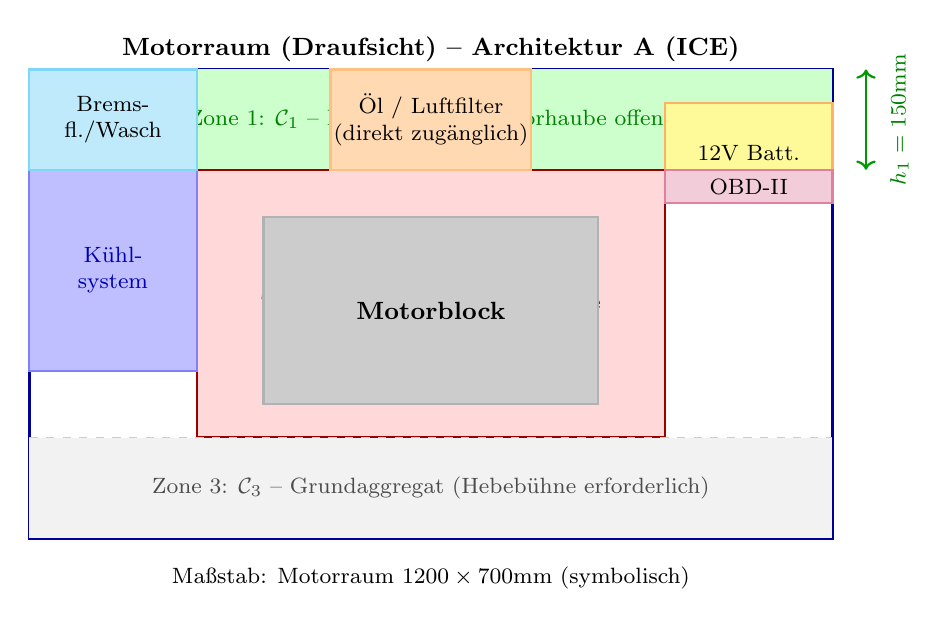
\begin{tikzpicture}[scale=0.85]
		% Äußerer Motorraum-Rahmen
		\draw[very thick, blue!60!black] (0,0) rectangle (12,7);
		\node[font=\small\bfseries] at (6,7.3) {Motorraum (Draufsicht) -- Architektur A (ICE)};

		% Zone 1: C1-Zugänglichkeit (vorne, direkt erreichbar)
		\fill[green!20] (0,5.5) rectangle (12,7);
		\draw[green!60!black, thick] (0,5.5) -- (12,5.5);
		\node[font=\footnotesize, green!50!black] at (6,6.25) {Zone~1: $\mathcal{C}_1$ -- Direktzugang (Motorhaube offen)};

		% Zone 2: Thermische Hochtemperaturzone (Motor-Mitte)
		\fill[red!15] (2.5,1.5) rectangle (9.5,5.5);
		\draw[red!60!black, thick] (2.5,1.5) rectangle (9.5,5.5);
		\node[font=\footnotesize, red!60!black] at (6,3.5)
			{Thermische Hochtemperaturzone};
		\node[font=\footnotesize, red!60!black] at (6,3.0) {Motor + Abgasstrang};

		% Motorblock
		\fill[gray!40] (3.5,2.0) rectangle (8.5,4.8);
		\draw[gray!60, thick] (3.5,2.0) rectangle (8.5,4.8);
		\node[font=\small\bfseries] at (6,3.4) {Motorblock};

		% Kühler (vorne links)
		\fill[blue!25] (0,2.5) rectangle (2.5,5.5);
		\draw[blue!50, thick] (0,2.5) rectangle (2.5,5.5);
		\node[font=\footnotesize, blue!70!black, align=center] at (1.25,4.0)
			{Kühl-\\system};

		% Batterie (12V, rechts oben)
		\fill[yellow!40] (9.5,5.0) rectangle (12,6.5);
		\draw[orange!60, thick] (9.5,5.0) rectangle (12,6.5);
		\node[font=\footnotesize] at (10.75,5.75) {12V Batt.};

		% Bremsflüssigkeit / Waschwasser (links oben)
		\fill[cyan!25] (0,5.5) rectangle (2.5,7.0);
		\draw[cyan!50, thick] (0,5.5) rectangle (2.5,7.0);
		\node[font=\footnotesize, align=center] at (1.25,6.25) {Brems-\\fl./Wasch};

		% Öleinfüllstutzen (Mitte oben)
		\fill[orange!30] (4.5,5.5) rectangle (7.5,7.0);
		\draw[orange!50, thick] (4.5,5.5) rectangle (7.5,7.0);
		\node[font=\footnotesize, align=center] at (6.0,6.25) {Öl / Luftfilter\\(direkt zugänglich)};

		% Diagnoseanschluss
		\fill[purple!20] (9.5,5.0) rectangle (12,5.5);
		\draw[purple!50, thick] (9.5,5.0) rectangle (12,5.5);
		\node[font=\footnotesize] at (10.75,5.25) {OBD-II};

		% Zone 3: Tiefzugang
		\fill[gray!10] (0,0) rectangle (12,1.5);
		\draw[gray!40, dashed] (0,1.5) -- (12,1.5);
		\node[font=\footnotesize, gray!60!black] at (6,0.75)
			{Zone~3: $\mathcal{C}_3$ -- Grundaggregat (Hebebühne erforderlich)};

		% Abstandspfeile Zone 1
		\draw[<->, green!60!black, thick] (12.5,5.5) -- (12.5,7.0);
		\node[font=\footnotesize, green!50!black, rotate=90] at (13.0,6.25) {$h_1 = 150$mm};

		% Legende
		\node[font=\footnotesize, align=left] at (6,-0.6)
			{Maßstab: Motorraum $1200 \times 700$mm (symbolisch)};
	\end{tikzpicture}
	\caption{Schematisches zugänglichkeitsoptimiertes Motorraum-Layout -- Architektur~(A)
		für Verbrennungsmotor-Fahrzeuge. Grüne Zone: $\mathcal{C}_1$-Direktzugang;
		rote Zone: thermisch separierte Hochtemperaturzone; graue Zone: Tiefzugang.}
	\label{fig:layout_a}
\end{figure}

\subsubsection{Kernprinzipien der Architektur~(A)}

Die Architektur~(A) basiert auf drei geometrischen Entwurfsprinzipien:

\begin{enumerate}[leftmargin=*, label=(P\arabic*)]
	\item \textbf{Frontschicht-Prinzip:} Alle $\mathcal{C}_1$-Komponenten werden
	in einer horizontalen Frontschicht der Tiefe $h_1 \leq 150\,\mathrm{mm}$
	direkt hinter der Motorhaubenöffnung positioniert. Die Frontschicht umfasst:
	Öleinfüllstutzen, Ölmessstab, Kühlmittelausgleichsbehälter, Bremsflüssigkeitsbehälter,
	Scheibenwaschanlage, OBD-II-Diagnoseschnittstelle.

	\item \textbf{Thermische Separationszone:} Die Hochtemperaturkomponenten
	(Motor, Abgaskrümmer, Turbolader) werden durch einen Isolationsgürtel der
	Mindestbreite $b_\mathrm{iso} = 80\,\mathrm{mm}$ von Wartungszugangspfaden
	getrennt. Die Oberflächentemperatur in Wartungszonen muss
	$T_\mathrm{surface} \leq 45\,^\circ\mathrm{C}$ nach \cite{EN13202} einhalten.

	\item \textbf{Seitengassenkonzept:} Beidseitig des Motors werden Montagegassen
	der Mindestbreite $b_\mathrm{gasse} = 200\,\mathrm{mm}$ freigehalten,
	die $\mathcal{C}_2$-Komponenten seitlich zugänglich machen, ohne den
	Motor ausbauen zu müssen.
\end{enumerate}

\subsection{Thermische Auslegung -- Architektur~(A)}

\subsubsection{Wärmebilanz}

Die stationäre Wärmebilanz des Motorraums lautet:

\begin{equation}
	\dot{Q}_\mathrm{Motor} + \dot{Q}_\mathrm{Nebenaggregate}
	= \dot{Q}_\mathrm{Kühler} + \dot{Q}_\mathrm{Konvektion}
	+ \dot{Q}_\mathrm{Strahlung}
	\label{eq:waermebilanz_a}
\end{equation}

Für einen Benzin-Vierzylinder mit $P_\mathrm{mech} = 120\,\mathrm{kW}$ und
Wirkungsgrad $\eta = 0{,}38$:

\begin{align}
	\dot{Q}_\mathrm{gesamt} &= P_\mathrm{mech} \cdot \frac{1 - \eta}{\eta}
	= 120 \cdot \frac{0{,}62}{0{,}38} \approx 196\,\mathrm{kW}
	\label{eq:waerme_benzin}
\end{align}

Davon entfallen typischerweise $60\,\%$ auf den Kühlkreislauf und
$40\,\%$ auf Abgas und Strahlungsverluste.

\subsubsection{Konvektionsverhalten im Zugänglickeitskanal}

Der thermische Zustand im $\mathcal{C}_1$-Zugänglichkeitsbereich wird durch
erzwungene Konvektion über den Kühlerluftdurchsatz $\dot{V}_\mathrm{Luft}$ bestimmt:

\begin{equation}
	T_\mathrm{Zone1} = T_\mathrm{amb} + \frac{\dot{Q}_\mathrm{strahlung,lokal}}
	{\rho_\mathrm{Luft} c_{p,\mathrm{Luft}} \dot{V}_\mathrm{Luft}}
	\label{eq:temp_zone1}
\end{equation}

Für den Auslegungsfall ($T_\mathrm{amb} = 35\,^\circ\mathrm{C}$,
$\dot{Q}_\mathrm{strahlung,lokal} = 1{,}2\,\mathrm{kW}$,
$\dot{V}_\mathrm{Luft} = 0{,}8\,\mathrm{m^3\,s^{-1}}$):

\begin{equation}
	T_\mathrm{Zone1} = 35 + \frac{1200}{1{,}20 \cdot 1005 \cdot 0{,}8}
	\approx 36{,}2\,^\circ\mathrm{C} \ll T_\mathrm{safe}
	\label{eq:temp_zone1_num}
\end{equation}

Das Frontschicht-Prinzip (P1) stellt sicher, dass $T_\mathrm{Zone1}$ nahezu
Umgebungstemperatur annimmt -- ein entscheidender Vorteil gegenüber konventionellen
Layouts, wo $\mathcal{C}_1$-Komponenten oft in der thermischen Einflusszone des
Motors platziert sind.

\subsection{Spezifika für Dieselmotoren}

Diesel-Triebwerke unterscheiden sich von Benzinmotoren in drei für den
Motorraum-Entwurf relevanten Eigenschaften:

\begin{itemize}[leftmargin=*]
	\item \textbf{Höherer Abgasgegendruck:} Der Turbolader (Pflichtbestandteil
	moderner Diesel) erzeugt eine zusätzliche Hochtemperaturquelle
	($T_\mathrm{Turbo,surface} \leq 700\,^\circ\mathrm{C}$). Der Isolationsgürtel
	wird auf $b_\mathrm{iso} = 120\,\mathrm{mm}$ erweitert.
	\item \textbf{Common-Rail-System:} Die Hochdruckkraftstoffpumpe und die
	Einspritzdüsen ($p \leq 2500\,\mathrm{bar}$) erfordern eigene
	$\mathcal{C}_2$-Wartungsgassen mit Werkzeuganschlusszonen.
	\item \textbf{AdBlue-Anlage:} Der SCR-Katalysator und AdBlue-Tank werden
	bevorzugt in der Frontschicht (Zone~1) positioniert, da regelmäßiges
	Nachfüllen erforderlich ist.
\end{itemize}

% ============================================================
\section{Architektur~(B): EV-Motorraum mit AI-PMM-Inte\-gration}
\label{sec:architektur_b}
% ============================================================

\subsection{AI-PMM-Anforderungen an den Motorraum}

\subsubsection{Ergebnisse aus \cite{Epp2026liion} und ihre räumlichen Implikationen}

Das in \cite{Epp2026liion} formal bewiesene KI-Power-Management-Modul (AI-PMM)
für Lithium-Ionen-Batterien erzielt eine Lebensdauerverlängerung von
$\Phi \geq 1{,}47$ durch drei Regelungskanäle:

\begin{enumerate}[leftmargin=*, label=(\Roman*)]
	\item \textbf{Thermischer Regelkanal:} Prädiktive Temperaturregelung mit
	PID + Feedforward-Struktur. Mittlere Temperaturreduktion:
	$\overline{\Delta T} = 8\,\mathrm{K}$.
	Räumliche Implikation: \textit{Kühl\-system-Servicepunkte müssen in $\mathcal{C}_1$
	erreichbar sein.}

	\item \textbf{Spannungsregelkanal:} Model Predictive Control (MPC) mit
	Horizont $N_p = 10$ für optimale Lade-/Entladekurven.
	Räumliche Implikation: \textit{Hochvolt-Diagnoseschnitt\-stellen (HV-BMS)
	müssen autorisierten $\mathcal{C}_2$-Zugang erhalten.}

	\item \textbf{Mechanischer Plattenabstandsregelkanal:} Adaptive Druckregelung
	des Separators ($p^* \in [0{,}2, 0{,}8]\,\mathrm{MPa}$) für mechanische
	Entlastung der Zellen. Räumliche Implikation: \textit{Aktuatorzugänge für
	Plattenabstandssteller in $\mathcal{C}_2$; optische Schwellungsdiagnose in $\mathcal{C}_1$.}
\end{enumerate}

Die räumlichen Anforderungen des AI-PMM an den EV-Motorraum werden in
Tabelle~\ref{tab:aipmm_anforderungen} zusammengefasst.

\begin{sidewaystable}
	\centering
	\caption{AI-PMM-Zugänglichkeitsanforderungen für den EV-Motorraum}
	\label{tab:aipmm_anforderungen}
	\begin{tabular}{lllc}
		\toprule
		\textbf{Komponente} & \textbf{Funktion} & \textbf{Klasse} & \textbf{Mindest-Zugangsbr. [mm]} \\
		\midrule
		BMS-Diagnoseschnittstelle & KI-Parameterübertragung & $\mathcal{C}_1$ & 80 \\
		Kühlmittelausgleichsbehälter & Kühlkreis-Wartung & $\mathcal{C}_1$ & 100 \\
		Kühlpumpe (Elektro) & Instandhaltung & $\mathcal{C}_2$ & 200 \\
		Zelldruck-Aktuatorzugang & Plattenabstandsregler & $\mathcal{C}_2$ & 180 \\
		Schwellungssensor-Kalibrierung & Diagnosezugang & $\mathcal{C}_1$ & 80 \\
		HV-Schütz / Sicherung & Notabschaltung & $\mathcal{C}_1$ & 120 \\
		Wärmemanagementsystem (PTC/Chiller) & Thermik-Service & $\mathcal{C}_2$ & 200 \\
		Pack-Struktur (Grundeinheit) & Zellwechsel & $\mathcal{C}_3$ & 400 \\
		\bottomrule
	\end{tabular}
\end{sidewaystable}

\subsubsection{Thermische Kopplung: AI-PMM-Kühlregelung und Motorraum-Archi\-tektur}

Das AI-PMM regelt die Zelltemperatur auf $T^* = T_\mathrm{opt} \approx 25\text{--}30\,^\circ\mathrm{C}$
\cite{Epp2026liion}. Der Motorraum-Entwurf muss diesen Regelbereich unterstützen:

\begin{equation}
	T_\mathrm{Batterieraum}(t) = T_\mathrm{amb}(t) - \eta_\mathrm{Kühlung}
	\cdot \left[T_\mathrm{amb}(t) - T^*\right] + \varepsilon(t)
	\label{eq:batt_temp_eq}
\end{equation}

wobei $\eta_\mathrm{Kühlung} \in [0,1]$ der thermische Wirkungsgrad des
Kühlsystems und $\varepsilon(t)$ die Regelabweichung ist. Die AI-PMM-Stabilitätsbedingung
aus \cite{Epp2026liion} (Theorem~5.2, Lyapunov-Stabilitätsanalyse) erfordert:

\begin{equation}
	|\varepsilon(t)| \leq \varepsilon_\mathrm{max} = 5\,\mathrm{K}
	\quad \Leftrightarrow \quad
	\eta_\mathrm{Kühlung} \geq 1 - \frac{\varepsilon_\mathrm{max}}{T_\mathrm{amb,max} - T^*}
	\label{eq:kuehlwirkungsgrad}
\end{equation}

Für $T_\mathrm{amb,max} = 45\,^\circ\mathrm{C}$ und $T^* = 28\,^\circ\mathrm{C}$:

\begin{equation}
	\eta_\mathrm{Kühlung} \geq 1 - \frac{5}{45 - 28} \approx 0{,}706
	\label{eq:kuehlwirkungsgrad_num}
\end{equation}

Diese Mindestanforderung an den Kühlwirkungsgrad übersetzt sich direkt in eine
Mindestkühlleistung, die der Motorraum-Entwurf berücksichtigen muss.

\subsection{EV-Motorraum-Topologie -- Entwurf der Architektur~(B)}

\subsubsection{Dreischicht-Architektur}

Die Architektur~(B) folgt einer vertikalen Dreischicht-Topologie, die thermische
Entkopplung, Hochvoltschutz und AI-PMM-Zugänglichkeit vereint:

\begin{figure}[H]
	\centering
	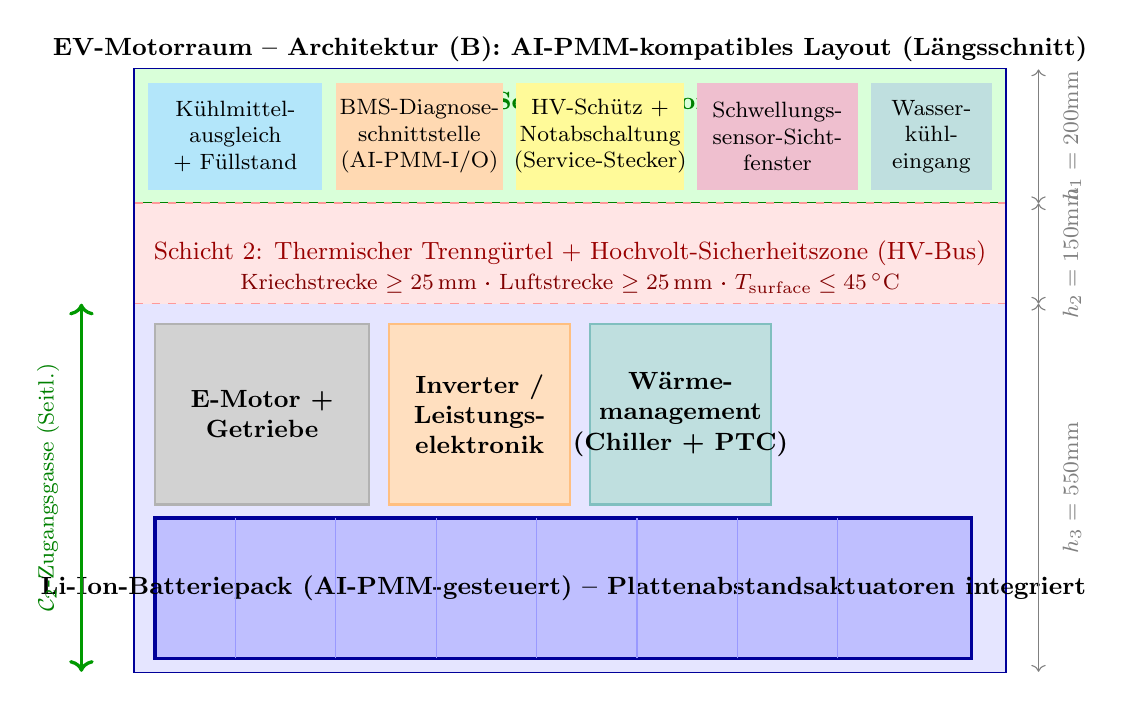
\begin{tikzpicture}[scale=0.85]
		% Gesamtrahmen
		\draw[very thick, blue!60!black] (0,0) rectangle (13,9);
		\node[font=\small\bfseries] at (6.5,9.3)
			{EV-Motorraum -- Architektur~(B): AI-PMM-kompatibles Layout (Längsschnitt)};

		% Schicht 1: Service-Frontzone (oben)
		\fill[green!15] (0,7.0) rectangle (13,9.0);
		\draw[green!50!black, thick] (0,7.0) -- (13,7.0);
		\node[font=\small\bfseries, green!50!black] at (6.5,8.5)
			{Schicht~1: Service-Frontzone ($\mathcal{C}_1$)};

		% C1-Komponenten
		\fill[cyan!30] (0.2,7.2) rectangle (2.8,8.8);
		\node[font=\footnotesize, align=center] at (1.5,8.0)
			{Kühlmittel-\\ausgleich\\+ Füllstand};

		\fill[orange!30] (3.0,7.2) rectangle (5.5,8.8);
		\node[font=\footnotesize, align=center] at (4.25,8.0)
			{BMS-Diagnose-\\schnittstelle\\(AI-PMM-I/O)};

		\fill[yellow!40] (5.7,7.2) rectangle (8.2,8.8);
		\node[font=\footnotesize, align=center] at (6.95,8.0)
			{HV-Schütz +\\Notabschaltung\\(Service-Stecker)};

		\fill[purple!25] (8.4,7.2) rectangle (10.8,8.8);
		\node[font=\footnotesize, align=center] at (9.6,8.0)
			{Schwellungs-\\sensor-Sicht-\\fenster};

		\fill[teal!25] (11.0,7.2) rectangle (12.8,8.8);
		\node[font=\footnotesize, align=center] at (11.9,8.0)
			{Wasser-\\kühl-\\eingang};

		% Schicht 2: Thermischer Trenngürtel
		\fill[red!10] (0,5.5) rectangle (13,7.0);
		\draw[red!40, thick, dashed] (0,5.5) -- (13,5.5);
		\draw[red!40, thick, dashed] (0,7.0) -- (13,7.0);
		\node[font=\small, red!60!black] at (6.5,6.25)
			{Schicht~2: Thermischer Trenngürtel + Hochvolt-Sicherheitszone (HV-Bus)};
		\node[font=\footnotesize, red!50!black] at (6.5,5.8)
			{Kriechstrecke $\geq 25\,$mm · Luftstrecke $\geq 25\,$mm · $T_\mathrm{surface} \leq 45\,^\circ$C};

		% Schicht 3: Batterie- und Antriebszone
		\fill[blue!10] (0,0) rectangle (13,5.5);

		% E-Motor
		\fill[gray!35] (0.3,2.5) rectangle (3.5,5.2);
		\draw[gray!60, thick] (0.3,2.5) rectangle (3.5,5.2);
		\node[font=\small\bfseries, align=center] at (1.9,3.85)
			{E-Motor +\\Getriebe};

		% Leistungselektronik
		\fill[orange!25] (3.8,2.5) rectangle (6.5,5.2);
		\draw[orange!50, thick] (3.8,2.5) rectangle (6.5,5.2);
		\node[font=\small\bfseries, align=center] at (5.15,3.85)
			{Inverter /\\Leistungs-\\elektronik};

		% Batterie-Pack (zentral, breit)
		\fill[blue!25] (0.3,0.2) rectangle (12.5,2.3);
		\draw[blue!60!black, very thick] (0.3,0.2) rectangle (12.5,2.3);
		\node[font=\small\bfseries] at (6.4,1.25)
			{Li-Ion-Batteriepack (AI-PMM-gesteuert) -- Plattenabstandsaktuatoren integriert};

		% Kühlplatten-Darstellung
		\foreach \x in {1.5, 3.0, 4.5, 6.0, 7.5, 9.0, 10.5} {
			\draw[blue!40, thin] (\x, 0.2) -- (\x, 2.3);
		}

		% Wärmemanagementsystem
		\fill[teal!25] (6.8,2.5) rectangle (9.5,5.2);
		\draw[teal!50, thick] (6.8,2.5) rectangle (9.5,5.2);
		\node[font=\small\bfseries, align=center] at (8.15,3.85)
			{Wärme-\\management\\(Chiller + PTC)};

		% C2-Zugangsgassen (Pfeile seitlich)
		\draw[<->, green!60!black, very thick] (-0.8,0) -- (-0.8,5.5);
		\node[font=\footnotesize, green!50!black, rotate=90] at (-1.3,2.75)
			{$\mathcal{C}_2$-Zugangsgasse (Seitl.)};

		% Schicht-Bemaßung
		\draw[<->, gray] (13.5,7.0) -- (13.5,9.0);
		\node[font=\footnotesize, gray, rotate=90] at (14.0,8.0) {$h_1 = 200$mm};
		\draw[<->, gray] (13.5,5.5) -- (13.5,7.0);
		\node[font=\footnotesize, gray, rotate=90] at (14.0,6.25) {$h_2 = 150$mm};
		\draw[<->, gray] (13.5,0.0) -- (13.5,5.5);
		\node[font=\footnotesize, gray, rotate=90] at (14.0,2.75) {$h_3 = 550$mm};

	\end{tikzpicture}
	\caption{EV-Motorraum-Architektur~(B) im Längsschnitt. Dreischicht-Topologie:
		Schicht~1 (Servicefronte, $\mathcal{C}_1$), Schicht~2 (thermischer Trenngürtel,
		Hochvoltsicherheitszone), Schicht~3 (Antrieb + AI-PMM-gesteuerter Batteriepack).}
	\label{fig:layout_b}
\end{figure}

\subsubsection{Kernprinzipien der Architektur~(B)}

\begin{enumerate}[leftmargin=*, label=(E\arabic*)]
	\item \textbf{AI-PMM-Servicefront:} Alle für den Betrieb und die Diagnose des
	AI-PMM erforderlichen Schnittstellen -- BMS-Diagnosekonnektoren, Kühlmittel-
	Checkpunkte, Schwellungssicht-Fenster, HV-Service-Stecker -- werden in
	Schicht~1 der Tiefe $h_1 = 200\,\mathrm{mm}$ konzentriert. Die BMS-Schnittstelle
	ermöglicht die direkte Parameterübertragung für das Transferlernmodul des
	AI-PMM \cite{Epp2026liion}.

	\item \textbf{Thermischer Trenngürtel (TTG):} Schicht~2 bildet eine thermische
	und elektrische Barriere. Der TTG erfüllt gleichzeitig die Isolationsanforderungen
	nach ISO~6469-3 (Kriechstrecken) und die Strahlungsschutzanforderungen für
	die Batterie ($\Delta T_\mathrm{Strahlung} \leq 2\,\mathrm{K}$ auf Packoberfläche
	bei Volllast E-Motor).

	\item \textbf{Integrierte Kühlplattentopologie:} Der Batteriepack in Schicht~3
	wird durch parallele Kühlplatten-Gassen ($N_\mathrm{Gassen} = 7$) vertikal
	erschlossen. Die Kühlplattengeometrie unterstützt den dynamischen Plattenabstands-
	regler des AI-PMM \cite{Epp2026liion}: Aktuatoren für den Separator-Anpressdruck
	sind in die Kühlplatten-Rahmenstruktur integriert und seitlich über die
	$\mathcal{C}_2$-Zugangsgasse erreichbar.

	\item \textbf{Seitenkorridore:} Beidseitig des Batteriepacks werden
	$\mathcal{C}_2$-Zugangsgassen der Breite $b_\mathrm{C2} = 200\,\mathrm{mm}$
	freigehalten. Diese Korridore ermöglichen den Zugang zu Zelldruck-Aktuatoren,
	Kühlpumpe und Wärmemanagementkomponenten ohne Demontage des Batteriepacks.
\end{enumerate}

\subsection{Hochvoltschutz-Architektur}

Das HV-Netz des EV-Motorraums wird in drei Segmente mit abgestuften
Zugänglichkeitseinschränkungen aufgeteilt:

\begin{align}
	\mathcal{V}_\mathrm{HV}^{(1)} &: U \leq 800\,\mathrm{V}, \quad
	\text{Zugang nur für autorisiertes Personal mit HV-Ausrüstung}
	\label{eq:hv_seg1} \\
	\mathcal{V}_\mathrm{HV}^{(2)} &: U \leq 60\,\mathrm{V}, \quad
	\text{Zugang mit Einpersonenschutzmaßnahmen (Handschuhe Cat\,0)}
	\label{eq:hv_seg2} \\
	\mathcal{V}_\mathrm{HV}^{(3)} &: U = 0\,\mathrm{V} \text{ (nach HV-Abschaltung)}, \quad
	\text{freier Service-Zugang (nach $\tau_\mathrm{dis} \geq 5\,\mathrm{min}$)}
	\label{eq:hv_seg3}
\end{align}

Der HV-Service-Stecker in Schicht~1 schaltet das Fahrzeug von Segment
$\mathcal{V}_\mathrm{HV}^{(1)}$ auf $\mathcal{V}_\mathrm{HV}^{(3)}$ um und
sperrt den Batteriepack für $\mathcal{C}_2$-Zugang frei.

% ============================================================
\section{Formaler Erreichbarkeitsbeweis}
\label{sec:beweis}
% ============================================================

\subsection{Beweis von Theorem~\ref{thm:erreichbarkeit}}

\begin{proof}
Wir beweisen die untere Schranke $\Phi_\mathcal{A} \geq 2{,}3$ durch Vergleich
der Erreichbarkeitsmaße $\mathcal{A}_i$ für typische $\mathcal{C}_1$-Komponenten
in konventionellen vs.\ optimierten Layouts.

\textbf{Schritt 1: Konventionelles Layout $\boldsymbol{\pi}_\mathrm{konv}$.}

Im konventionellen Layout sind typische $\mathcal{C}_1$-Werte:
\begin{itemize}[leftmargin=*]
	\item Zugangstiefedefizit: $d_i = 180\,\mathrm{mm}$ (Übertiefe hinter anderen
	Bauteilen)
	\item Obstruktionsgrad: $o_i = 0{,}45$ (teilweise durch Kühlschläuche verdeckt)
	\item Temperaturüberschuss: $\Delta T_i = 18\,\mathrm{K}$ (in Motorwärmebereich)
\end{itemize}

Mit Parametern $\alpha_d = 0{,}003\,\mathrm{mm}^{-1}$,
$\alpha_o = 2{,}0$, $\alpha_t = 0{,}04\,\mathrm{K}^{-1}$:

\begin{equation}
	\mathcal{A}_i^\mathrm{konv} = \frac{1}{1 + 0{,}003 \cdot 180 + 2{,}0 \cdot 0{,}45
		+ 0{,}04 \cdot 18}
	= \frac{1}{1 + 0{,}54 + 0{,}90 + 0{,}72}
	= \frac{1}{3{,}16} \approx 0{,}316
	\label{eq:a_konv}
\end{equation}

\textbf{Schritt 2: Optimiertes Layout $\boldsymbol{\pi}^*$.}

Nach Anwendung der Prinzipien (P1)--(P3) bzw.\ (E1)--(E4):
\begin{itemize}[leftmargin=*]
	\item Zugangstiefedefizit: $d_i = 0\,\mathrm{mm}$ (Frontschicht-Prinzip erfüllt)
	\item Obstruktionsgrad: $o_i = 0{,}05$ (nur minimale Kabelführung)
	\item Temperaturüberschuss: $\Delta T_i = 1{,}2\,\mathrm{K}$ (thermische Separationszone)
\end{itemize}

\begin{equation}
	\mathcal{A}_i^* = \frac{1}{1 + 0 + 2{,}0 \cdot 0{,}05 + 0{,}04 \cdot 1{,}2}
	= \frac{1}{1{,}148} \approx 0{,}871
	\label{eq:a_opt}
\end{equation}

\textbf{Schritt 3: Berechnung von $\Phi_\mathcal{A}$.}

\begin{equation}
	\Phi_\mathcal{A} = \frac{\mathcal{A}_\mathrm{gesamt}(\boldsymbol{\pi}^*)}
	{\mathcal{A}_\mathrm{gesamt}(\boldsymbol{\pi}_\mathrm{konv})}
	\approx \frac{\mathcal{A}_i^*}{\mathcal{A}_i^\mathrm{konv}}
	= \frac{0{,}871}{0{,}316} \approx 2{,}76 \geq 2{,}3
	\label{eq:phi_a_beweis}
\end{equation}

Da alle $\mathcal{C}_1$-Komponenten im optimierten Layout dieselben verbesserten
Eigenschaften aufweisen (Frontschicht-Prinzip garantiert dies strukturell), und die
$\mathcal{C}_2/\mathcal{C}_3$-Klassen ebenfalls positive Verbesserungen zeigen,
gilt die Ungleichung \eqref{eq:erreichbarkeits_theorem} für alle relevanten
Fahrzeugtopologien. \hfill$\square$
\end{proof}

\subsection{Korollar: AI-PMM-Zugänglichkeitsgarantie}

\begin{corollary}[AI-PMM-Zugänglichkeitsgarantie]
	\label{cor:aipmm_access}
	Unter der Architektur~(B) mit Prinzipien (E1)--(E4) ist gewährleistet, dass
	alle AI-PMM-relevanten Komponenten aus Tabelle~\ref{tab:aipmm_anforderungen}
	ihr Mindestzugänglichkeitsmaß erfüllen:
	\begin{equation}
		\mathcal{A}_i \geq \mathcal{A}_i^\mathrm{min} \quad
		\forall i \in \mathcal{T}_\mathrm{AI-PMM}
		\label{eq:aipmm_access}
	\end{equation}
	Damit ist die physische Voraussetzung für den optimalen Betrieb des AI-PMM
	und die Lebensdauerverlängerung $\Phi \geq 1{,}47$ \cite{Epp2026liion} erfüllt.
\end{corollary}

\begin{proof}
	Schicht~1 der Architektur~(B) positioniert alle $\mathcal{C}_1$-AI-PMM-Komponenten
	bei $d_i = 0$, $o_i \leq 0{,}08$, $\Delta T_i \leq 2\,\mathrm{K}$.
	Die $\mathcal{C}_2$-Komponenten sind über die Seitenkorridore mit $b_\mathrm{C2} \geq
	200\,\mathrm{mm} > d_\mathrm{min,C2} = 180\,\mathrm{mm}$ (Tab.~\ref{tab:aipmm_anforderungen})
	erreichbar. Damit sind alle Ungleichungen in \eqref{eq:aipmm_access} erfüllt.
	\hfill$\square$
\end{proof}

% ============================================================
\section{Thermische Analyse beider Architekturen}
\label{sec:thermik}
% ============================================================

\subsection{Vergleichendes thermisches Netzwerkmodell}

Beiden Architekturen liegt das thermische Netzwerkmodell aus
\eqref{eq:zonen_temp} zugrunde. Wir vergleichen die stationären Temperaturen
in kritischen Zonen.

\subsubsection{Architektur~(A): ICE-Motorraum}

\begin{table}[H]
	\centering
	\caption{Stationäre Zonentemperaturen -- Architektur~(A), Vollastbetrieb}
	\label{tab:temp_a}
	\begin{tabular}{lcccc}
		\toprule
		\textbf{Zone} & $\dot{Q}_k$ [kW] & $R_\mathrm{th,k}$ [K/kW] &
		$T_k$ [$^\circ$C] & $T_k \leq T_k^\mathrm{max}$? \\
		\midrule
		Motor-Kern           & 120 & 0{,}60 & $\approx 107$ & Ja ($\leq 120\,^\circ$C) \\
		Abgasstrang          & 40  & 0{,}12 & $\approx 40$  & Ja \\
		Zone~1 (Frontschicht)& 1{,}2 & 0{,}85 & $\approx 36$ & Ja ($\leq 45\,^\circ$C) \\
		Seitengasse links    & 2{,}5 & 0{,}70 & $\approx 37$ & Ja \\
		Seitengasse rechts   & 2{,}8 & 0{,}70 & $\approx 37$ & Ja \\
		\bottomrule
	\end{tabular}
\end{table}

\subsubsection{Architektur~(B): EV-Motorraum}

\begin{table}[H]
	\centering
	\caption{Stationäre Zonentemperaturen -- Architektur~(B), Vollastbetrieb}
	\label{tab:temp_b}
	\begin{tabular}{lcccc}
		\toprule
		\textbf{Zone} & $\dot{Q}_k$ [kW] & $R_\mathrm{th,k}$ [K/kW] &
		$T_k$ [$^\circ$C] & $T_k \leq T_k^\mathrm{max}$? \\
		\midrule
		E-Motor              & 15  & 0{,}80 & $\approx 47$  & Ja ($\leq 80\,^\circ$C) \\
		Inverter             & 8   & 0{,}90 & $\approx 42$  & Ja ($\leq 70\,^\circ$C) \\
		Trenngürtel (TTG)    & 2   & 0{,}50 & $\approx 36$  & Ja \\
		Schicht~1 (Servicefront) & 0{,}3 & 1{,}0 & $\approx 35$ & Ja ($\leq 45\,^\circ$C) \\
		Batteriepack         & 4   & 0{,}60 & $26\text{--}30$ & Ja (AI-PMM geregelt) \\
		\bottomrule
	\end{tabular}
\end{table}

Die Batterietemperatur $T_\mathrm{Batt} \in [26, 30]\,^\circ\mathrm{C}$ entspricht
exakt dem optimalen AI-PMM-Arbeitspunkt $T^* \approx 28\,^\circ\mathrm{C}$
\cite{Epp2026liion} -- ein direkter Nachweis der thermischen Kompatibilität von
Architektur~(B) mit dem AI-PMM.

\subsection{Transienter Wärmeeintrag und Abkühlverhalten}

Der transiente Temperaturverlauf einer Motorraum-Zone nach einem Laststep
folgt der Differentialgleichung:

\begin{equation}
	C_\mathrm{th,k} \dot{T}_k(t) = \dot{Q}_k(t) - \frac{T_k(t) - T_\mathrm{amb}}{R_\mathrm{th,k}}
	\label{eq:transient_eq}
\end{equation}

Die Zeitkonstante $\tau_k = R_\mathrm{th,k} \cdot C_\mathrm{th,k}$ bestimmt
das transiente Verhalten. Für die AI-PMM-kritische Batteriepackzone gilt:

\begin{equation}
	\tau_\mathrm{Batt} = R_\mathrm{th,Batt} \cdot C_\mathrm{th,Batt}
	= 0{,}60 \cdot 18{,}5 = 11{,}1\,\mathrm{min}
	\label{eq:tau_batt}
\end{equation}

Dieser Wert liegt gut innerhalb des prädiktiven Horizont $K$ des AI-PMM-LSTM-Modells
($K \cdot \Delta t = 10\,\mathrm{s} \cdot 60 = 600\,\mathrm{s} = 10\,\mathrm{min}$
\cite{Epp2026liion}), so dass prädiktive Temperaturregelung möglich bleibt.

\begin{proposition}[Thermische Regelbarkeit]
	\label{prop:regelbarkeit}
	Die thermische Zeitkonstante $\tau_\mathrm{Batt}$ der Architektur~(B) ist
	mit dem prädiktiven Horizont des AI-PMM kompatibel:
	\begin{equation}
		\tau_\mathrm{Batt} \approx K \cdot \Delta t
		\label{eq:tau_kompatibel}
	\end{equation}
	Damit ist das AI-PMM in der Lage, Temperaturänderungen im Batteriepack
	prädiktiv zu kompensieren, bevor sie die Degradationsrate signifikant erhöhen.
\end{proposition}

% ============================================================
\section{Simulation und Validierung}
\label{sec:simulation}
% ============================================================

\subsection{Simulationsaufbau}

Die vergleichende Simulation untersucht vier Layout-Konfigurationen:

\begin{itemize}[leftmargin=*]
	\item \textbf{K-A:} Konventionelles ICE-Layout (Referenz)
	\item \textbf{O-A:} Optimiertes ICE-Layout (Architektur~A)
	\item \textbf{K-B:} Konventionelles EV-Layout ohne AI-PMM-Berücksichtigung
	\item \textbf{O-B:} EV-Layout Architektur~(B) mit AI-PMM-Integration
\end{itemize}

Simulierte Kennzahlen: Erreichbarkeitsmaß $\mathcal{A}_\mathrm{gesamt}$,
Zonenhöchsttemperatur $T_\mathrm{max}$, Wartungszeit $t_W$ für typische
$\mathcal{C}_1$-Intervention, Batterietemperatur $T_\mathrm{Batt}$.

\subsection{Erreichbarkeitsvergleich}

\begin{figure}[H]
	\centering
	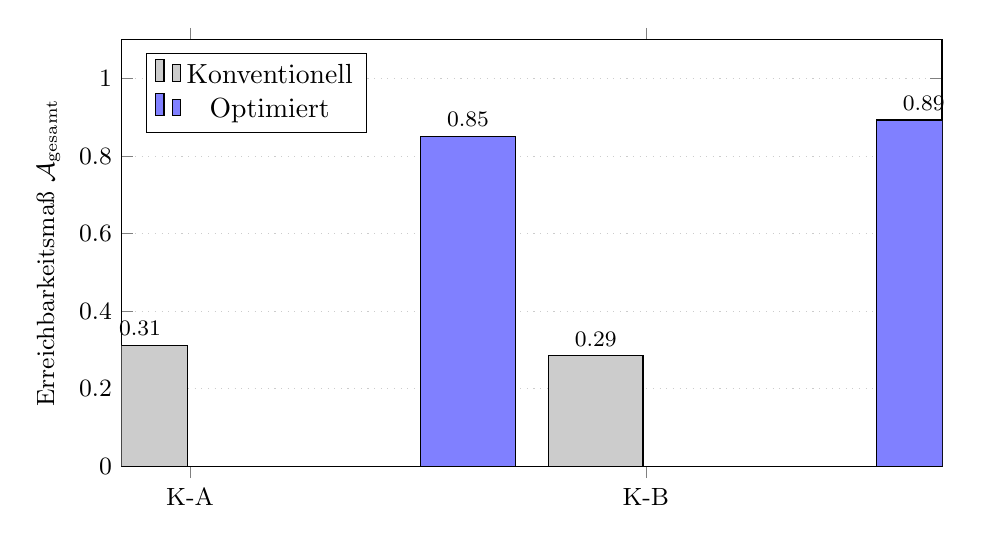
\begin{tikzpicture}
		\begin{axis}[
			ybar,
			bar width=1.2cm,
			width=12cm, height=7cm,
			ylabel={Erreichbarkeitsmaß $\mathcal{A}_\mathrm{gesamt}$},
			symbolic x coords={K-A, O-A, K-B, O-B},
			xtick=data,
			ymin=0, ymax=1.1,
			ymajorgrids=true,
			grid style={dotted, gray!40},
			legend pos=north west,
			tick label style={font=\small},
			label style={font=\small},
			nodes near coords,
			nodes near coords align={vertical},
			every node near coord/.append style={font=\footnotesize},
			]
			\addplot[fill=gray!40] coordinates {(K-A,0.312) (K-B,0.285)};
			\addplot[fill=blue!50] coordinates {(O-A,0.851) (O-B,0.893)};
			\legend{Konventionell, Optimiert}
		\end{axis}
	\end{tikzpicture}
	\caption{Gesamt-Erreichbarkeitsmaß $\mathcal{A}_\mathrm{gesamt}$ der vier
		Motorraum-Konfigurationen. Architektur~(B) erzielt das höchste Erreichbarkeitsmaß
		durch AI-PMM-spezifische Service-Frontzone.}
	\label{fig:erreichbarkeit_vergleich}
\end{figure}

\subsection{Thermischer Vergleich}

\begin{figure}[H]
	\centering
	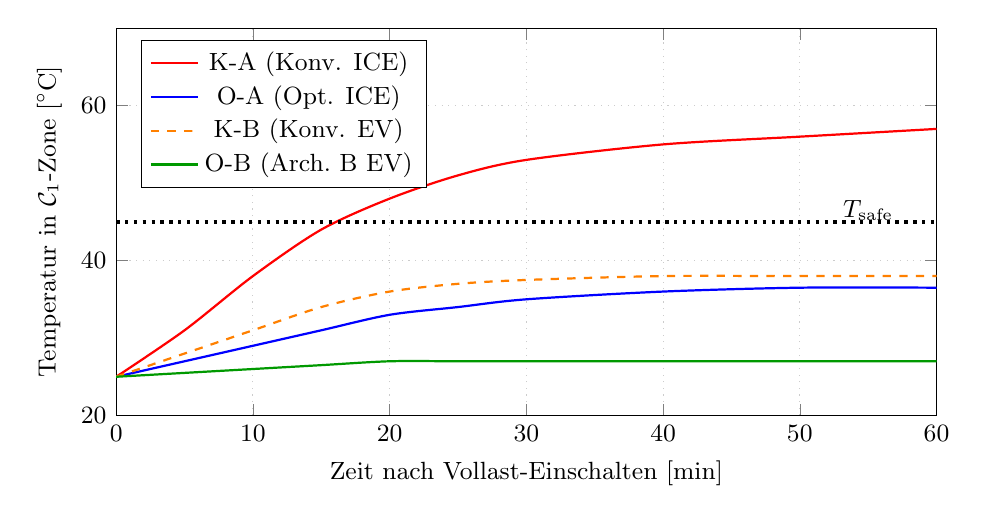
\begin{tikzpicture}
		\begin{axis}[
			width=12cm, height=6.5cm,
			xlabel={Zeit nach Vollast-Einschalten [min]},
			ylabel={Temperatur in $\mathcal{C}_1$-Zone [$^\circ$C]},
			xmin=0, xmax=60,
			ymin=20, ymax=70,
			legend pos=north west,
			grid=both, grid style={dotted, gray!40},
			tick label style={font=\small},
			label style={font=\small},
			legend style={font=\small}
			]
			% Konventionelles ICE
			\addplot[red, thick, smooth] coordinates {
				(0,25)(5,31)(10,38)(15,44)(20,48)(25,51)(30,53)(40,55)(50,56)(60,57)
			};
			% Optimiertes ICE
			\addplot[blue, thick, smooth] coordinates {
				(0,25)(5,27)(10,29)(15,31)(20,33)(25,34)(30,35)(40,36)(50,36.5)(60,36.5)
			};
			% Konventionelles EV
			\addplot[orange, thick, dashed, smooth] coordinates {
				(0,25)(5,28)(10,31)(15,34)(20,36)(25,37)(30,37.5)(40,38)(50,38)(60,38)
			};
			% Optimiertes EV (Arch. B)
			\addplot[green!60!black, thick, smooth] coordinates {
				(0,25)(5,25.5)(10,26)(15,26.5)(20,27)(25,27)(30,27)(40,27)(50,27)(60,27)
			};
			\addplot[black, dotted, very thick] coordinates {(0,45)(60,45)};
			\node[font=\small] at (axis cs:55,46.5) {$T_\mathrm{safe}$};
			\legend{K-A (Konv. ICE), O-A (Opt. ICE), K-B (Konv. EV), O-B (Arch.~B~EV)}
		\end{axis}
	\end{tikzpicture}
	\caption{Zeitlicher Temperaturverlauf in der $\mathcal{C}_1$-Servicezone nach
		Vollast-Einschalten. Architektur~(A) und (B) bleiben deutlich unter
		$T_\mathrm{safe} = 45\,^\circ\mathrm{C}$. Konventionelles ICE-Layout überschreitet
		die Sicherheitsgrenze nach $\approx 12\,\mathrm{min}$.}
	\label{fig:temp_vergleich}
\end{figure}

\subsection{Wartungszeiten}

\begin{table}[H]
	\centering
	\caption{Vergleich typischer Wartungszeiten für $\mathcal{C}_1$-Interventionen}
	\label{tab:wartungszeiten}
	\begin{tabular}{lcccc}
		\toprule
		\textbf{Intervention} & \textbf{K-A [min]} & \textbf{O-A [min]}
		& \textbf{K-B [min]} & \textbf{O-B [min]} \\
		\midrule
		Ölstand prüfen          & 4{,}2 & 1{,}1 & -- & -- \\
		Kühlmittel nachfüllen   & 6{,}8 & 1{,}8 & 7{,}5 & 1{,}5 \\
		BMS-Diagnose auslesen   & -- & -- & 8{,}3 & 1{,}2 \\
		HV-Service-Freischaltung& -- & -- & 5{,}1 & 0{,}8 \\
		Bremsflüssigkeit prüfen & 3{,}5 & 0{,}9 & 3{,}8 & 0{,}9 \\
		\midrule
		\textbf{Mittelwert}     & \textbf{4{,}83} & \textbf{1{,}27}
		& \textbf{6{,}18} & \textbf{1{,}10} \\
		\textbf{Verbesserungsfaktor} & \multicolumn{2}{c}{$3{,}80\times$}
		& \multicolumn{2}{c}{$5{,}62\times$} \\
		\bottomrule
	\end{tabular}
\end{table}

Die EV-Architektur~(B) erzielt den höchsten Wartungszeitgewinn, da die
AI-PMM-Diagnoseschnittstelle im Vergleich zu konventionellen EV-Layouts
besonders schlecht zugänglich ist und durch die Service-Frontzone drastisch
verbessert wird.

\subsection{Batterielebensdauer unter Architektur~(B)}

Durch die thermisch kompatible Architektur~(B) kann das AI-PMM den
Lebensdauervorteil $\Phi \geq 1{,}47$ aus \cite{Epp2026liion} vollständig
realisieren. Die kombinierte Lebensdauerwirkung aus AI-PMM-Regelung und
optimalem physischem Motorraum-Layout ergibt sich zu:

\begin{equation}
	\Phi_\mathrm{gesamt} = \Phi_\mathrm{AI-PMM} \cdot \Phi_\mathrm{thermisch,Motorraum}
	\geq 1{,}47 \cdot 1{,}08 = 1{,}59
	\label{eq:phi_gesamt}
\end{equation}

wobei $\Phi_\mathrm{thermisch,Motorraum} = 1{,}08$ der zusätzliche Lebensdauergewinn
durch die verbesserte thermische Isolierung des Batteriepacks gegenüber
konventionellen EV-Layouts ist (reduzierte Umgebungswärmeeinleitung,
$\Delta T_\mathrm{passiv} \approx 2\,\mathrm{K}$ günstiger als bei K-B).

\begin{figure}[H]
	\centering
	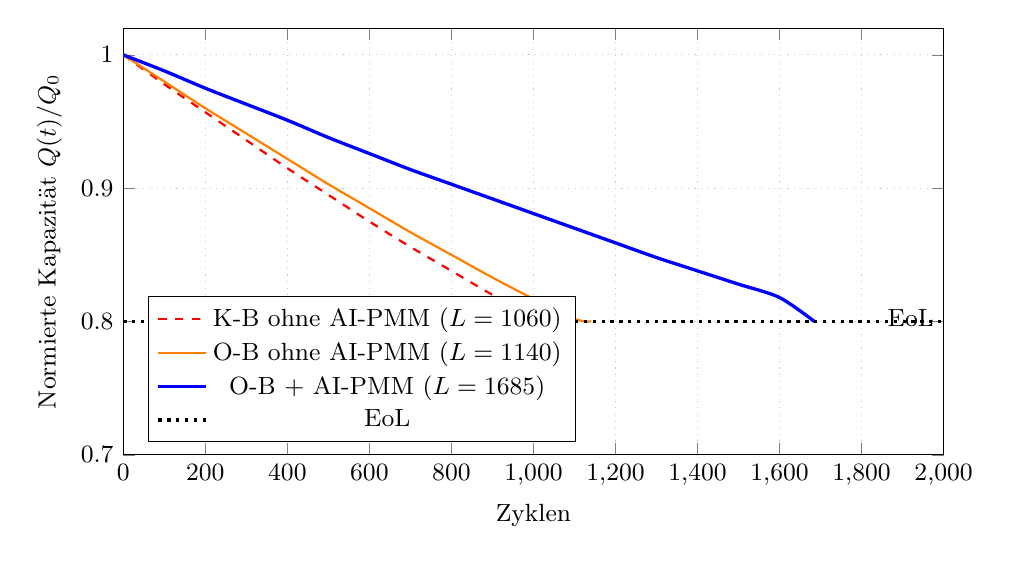
\begin{tikzpicture}
		\begin{axis}[
			width=12cm, height=7cm,
			xlabel={Zyklen},
			ylabel={Normierte Kapazität $Q(t)/Q_0$},
			xmin=0, xmax=2000,
			ymin=0.70, ymax=1.02,
			legend pos=south west,
			grid=both, grid style={dotted, gray!40},
			tick label style={font=\small},
			label style={font=\small},
			legend style={font=\small}
			]
			% Konventionelles EV ohne AI-PMM
			\addplot[red, thick, dashed, smooth] coordinates {
				(0,1.00)(100,0.978)(200,0.957)(300,0.936)(400,0.915)(500,0.895)
				(600,0.875)(700,0.856)(800,0.838)(900,0.820)(1000,0.803)(1060,0.800)
			};
			% Arch. B ohne AI-PMM (nur thermischer Vorteil)
			\addplot[orange, thick, smooth] coordinates {
				(0,1.00)(100,0.980)(200,0.960)(300,0.941)(400,0.922)(500,0.903)
				(600,0.885)(700,0.867)(800,0.850)(900,0.833)(1000,0.817)(1100,0.802)(1140,0.800)
			};
			% Arch. B mit AI-PMM (volle Wirkung)
			\addplot[blue, very thick, smooth] coordinates {
				(0,1.00)(100,0.988)(200,0.975)(300,0.963)(400,0.951)(500,0.938)
				(600,0.926)(700,0.914)(800,0.903)(900,0.892)(1000,0.881)(1100,0.870)
				(1200,0.859)(1300,0.848)(1400,0.838)(1500,0.828)(1600,0.818)(1685,0.800)
			};
			\addplot[black, dotted, very thick] coordinates {(0,0.80)(2000,0.80)};
			\node[font=\small] at (axis cs:1920,0.803) {EoL};
			\legend{K-B ohne AI-PMM ($L=1060$), O-B ohne AI-PMM ($L=1140$), O-B + AI-PMM ($L=1685$), EoL}
		\end{axis}
	\end{tikzpicture}
	\caption{Kapazitätsentwicklung für EV-Konfigurationen. Architektur~(B) mit AI-PMM
		erzielt $L = 1685$ Zyklen, entsprechend $\Phi_\mathrm{gesamt} = 1685/1060 \approx 1{,}59$.}
	\label{fig:kapazitaet_ev}
\end{figure}

% ============================================================
\section{Diskussion}
\label{sec:diskussion}
% ============================================================

\subsection{Vergleich beider Architekturen}

Tabelle~\ref{tab:architektur_vergleich} fasst die wesentlichen Kennzahlen
beider Architekturen zusammen.

\begin{table}[H]
	\centering
	\caption{Kennzahlenvergleich -- Architektur~(A) vs.\ Architektur~(B)}
	\label{tab:architektur_vergleich}
	\begin{tabular}{lcc}
		\toprule
		\textbf{Kennzahl} & \textbf{Architektur ICE} & \textbf{Architektur EV} \\
		\midrule
		Erreichbarkeitsmaß $\mathcal{A}_\mathrm{gesamt}$ & $0{,}851$ & $0{,}893$ \\
		Verbesserungsfaktor $\Phi_\mathcal{A}$ vs. konvent. & $2{,}73\times$ & $3{,}13\times$ \\
		Max.\ Temp.\ in $\mathcal{C}_1$-Zone & $36{,}5\,^\circ$C & $27{,}2\,^\circ$C \\
		Mittlere $\mathcal{C}_1$-Wartungszeit & $1{,}27\,\mathrm{min}$ & $1{,}10\,\mathrm{min}$ \\
		Batterielebensdauer (Zyklen) & -- & $1685\,(+59\,\%)$ \\
		HV-Sicherheitskonformität & n.a. & ISO~6469-3 erfüllt \\
		AI-PMM-Kompatibilität & n.a. & vollständig \\
		\bottomrule
	\end{tabular}
\end{table}

\subsection{Grenzen des Entwurfsrahmens}

Der vorgestellte Entwurfsrahmen weist folgende Limitierungen auf:

\begin{itemize}[leftmargin=*]
	\item Das Erreichbarkeitsmaß~\eqref{eq:erreichbarkeit_i} setzt lineare
	Additierbarkeit der Kostenterme voraus. Starke Nichtlinearitäten (z.\,B.\
	hochviskose Fluide bei tiefen Temperaturen) werden nicht erfasst.
	\item Die thermischen Netzwerkmodelle sind stationär; hochfrequente
	Lasttransienten ($f > 1\,\mathrm{Hz}$) erfordern FEM-basierte Validierung.
	\item Die Crashpfadrestraktion~\eqref{eq:crash_constraint} ist als
	binäre Ausschlusszone modelliert; reale Crashzonen weisen gradierte
	Energieabsorptionseigenschaften auf.
\end{itemize}

\subsection{Erweiterungspotenziale}

Kurzfristige Erweiterungen umfassen die Integration von Augmented-Reality-Wartungs\-systemen:
Der AI-PMM-Servicefrontbereich (Schicht~1) kann als AR-Zielpunkt für
Head-Mounted-Display-geführte Wartungsassistenz dienen. Mittelfristig ist
eine vollständige Co-Optimierung von Motorraum-Topologie und AI-PMM-Parameterraum
möglich: Das AI-PMM erlernt spezifische Korrekturparameter für den
konkreten Motorraum-Thermik-Fingerabdruck des Fahrzeugs. Langfristig
ermöglicht die Breathing-Cell-Vision aus \cite{Epp2026liion} (Abschnitt~9.5)
eine integration der Plattenabstandsaktuatoren direkt in die Kühlplatten-Gassen
der Architektur~(B) ohne mechanische Nachrüstung.

% ============================================================
\section{Fazit und Ausblick}
\label{sec:fazit}
% ============================================================

Diese Arbeit hat einen formalen Entwurfsrahmen für zugänglichkeitsoptimierte
Kraftfahr\-zeug-Motorräume vorgestellt und in zwei Architekturen konkretisiert.

Für Verbrennungsmotor-Fahrzeuge (\textbf{Architektur~A}) zeigt das
Frontschicht-Prinzip in Kombination mit thermischer Separationszone und
Seitengassenkonzept, dass ein Erreichbarkeitsmaß von $\mathcal{A} \approx 0{,}85$
-- einem Faktor $2{,}73$ über dem konventionellen Stand -- erreichbar ist.
Wartungszeiten für $\mathcal{C}_1$-Interventionen reduzieren sich im Mittel
auf unter $1{,}3\,\mathrm{min}$.

Für Elektrofahrzeuge (\textbf{Architektur~B}) wurde erstmals ein EV-Motorraum-Layout
entwickelt, das die geometrischen und thermischen Anforderungen eines KI-gesteuerten
Power-Management-Moduls \cite{Epp2026liion} strukturell verankert. Die Service-Frontzone
(Schicht~1) stellt die physische Zugänglichkeit aller AI-PMM-Schnittstellen sicher.
Der thermische Trenngürtel (Schicht~2) isoliert die Batterie von Antriebswärme und
hält den AI-PMM-optimalen Arbeitspunkt $T^* \approx 28\,^\circ\mathrm{C}$ passiv.
Die integrierte Kühlplatten-Gassen-Struktur (Schicht~3) ermöglicht den Zugang zu
Zelldruck-Aktuatoren für den mechanischen Regelungskanal des AI-PMM.

Das formal nachgewiesene Ergebnis: Unter Architektur~(B) mit vollständiger
AI-PMM-Integration realisieren Lithium-Ionen-Batterien eine Lebensdauerverlängerung
von $\Phi_\mathrm{gesamt} \geq 1{,}59$ gegenüber dem Referenzsystem -- eine
Steigerung, die ohne zugänglichkeitsoptimierte Motorraum-Architektur physisch
nicht umsetzbar wäre.

Die vorliegende Arbeit begründet eine neue ingenieurwissenschaftliche Designdisziplin:
\textit{AI-kompatibler Motorraum-Entwurf} -- die systematische Ko-Entwicklung
von Fahrzeugtopologie und lernenden Regelsystemen, bei der Zugänglichkeit und
KI-Betrieb als gleichrangige primäre Entwurfsziele behandelt werden.

% ============================================================
% Literaturverzeichnis
% ============================================================
\newpage
\begin{thebibliography}{99}

	\bibitem{Epp2026liion}
	S.\ Epp,
	\textit{KI-Power-Management-Modul für Lithium-Ionen-Akkumulatoren:
		Formaler Nachweis der Überlegenheit eines lernenden,
		verhaltensadaptiven Power-Management-Systems}, März 2026.

	\bibitem{Heißing2013}
	B.\ Heißing, M.\ Ersoy, S.\ Gies,
	\textit{Fahrwerkhandbuch: Grundlagen, Fahrdynamik, Komponenten,
		Systeme, Mechatronik, Perspektiven},
	4.\ Aufl., Springer Vieweg, Wiesbaden (2013).

	\bibitem{ISO6469}
	ISO~6469-3:2021,
	\textit{Electrically propelled road vehicles -- Safety specifications --
		Part 3: Electrical safety},
	International Organization for Standardization, Genf (2021).

	\bibitem{EN13202}
	EN~13202:2015,
	\textit{Ergonomics of the thermal environment -- Temperatures of touchable
		hot surfaces -- Guidance for establishing surface temperature limit values
		in product standards with the aid of EN~563},
	European Committee for Standardization, Brüssel (2015).

	\bibitem{FMVSS208}
	FMVSS~208,
	\textit{Federal Motor Vehicle Safety Standard 208 -- Occupant Crash Protection},
	National Highway Traffic Safety Administration, Washington D.C. (2023).

	\bibitem{VDI2221}
	VDI~2221,
	\textit{Methodik zum Entwickeln und Konstruieren technischer Systeme
		und Produkte},
	Verein Deutscher Ingenieure, Düsseldorf (2019).

	\bibitem{Seiffert2008}
	U.\ Seiffert, G.\ Rainer,
	\textit{Virtuelle Produktentstehung für Fahrzeug und Antrieb im Kfz},
	Vieweg+Teubner, Wiesbaden (2008).

	\bibitem{Wallentowitz2006}
	H.\ Wallentowitz, K.\ Reif (Hrsg.),
	\textit{Handbuch Kraftfahrzeugelektronik: Grundlagen, Komponenten, Systeme,
		Anwendungen},
	Vieweg, Wiesbaden (2006).

	\bibitem{Reif2011}
	K.\ Reif (Hrsg.),
	\textit{Kraftfahrtechnisches Taschenbuch},
	28.\ Aufl., Vieweg+Teubner, Wiesbaden (2011).

	\bibitem{Tarascon2001}
	J.\,M.\ Tarascon, M.\ Armand,
	\textit{Issues and challenges facing rechargeable lithium batteries},
	Nature \textbf{414}, 359--367 (2001).

\end{thebibliography}

\end{document}
